%%%%                %%%%
%%%% IMPLEMENTACIÓN %%%%
%%%%                %%%%

\chapter{Diseño e Implementación}
\label{chap:implemetación}

\lettrine{E}{ste} capítulo describe el diseño y la implementación de la solución construida. El sistema implementa un flujo de datos o pipeline. Toda la programación se ha realizado por medio de los lenguajes Python 3, C y Bash.

\section{Etapas del sistema}

Los datos son sometidos a un proceso por etapas tal como se ve en la figura \ref{fig:vision-general-del-sistema}. A continuación se detalla cada una de estas etapas.

\begin{figure}[hp!]
    \centering
    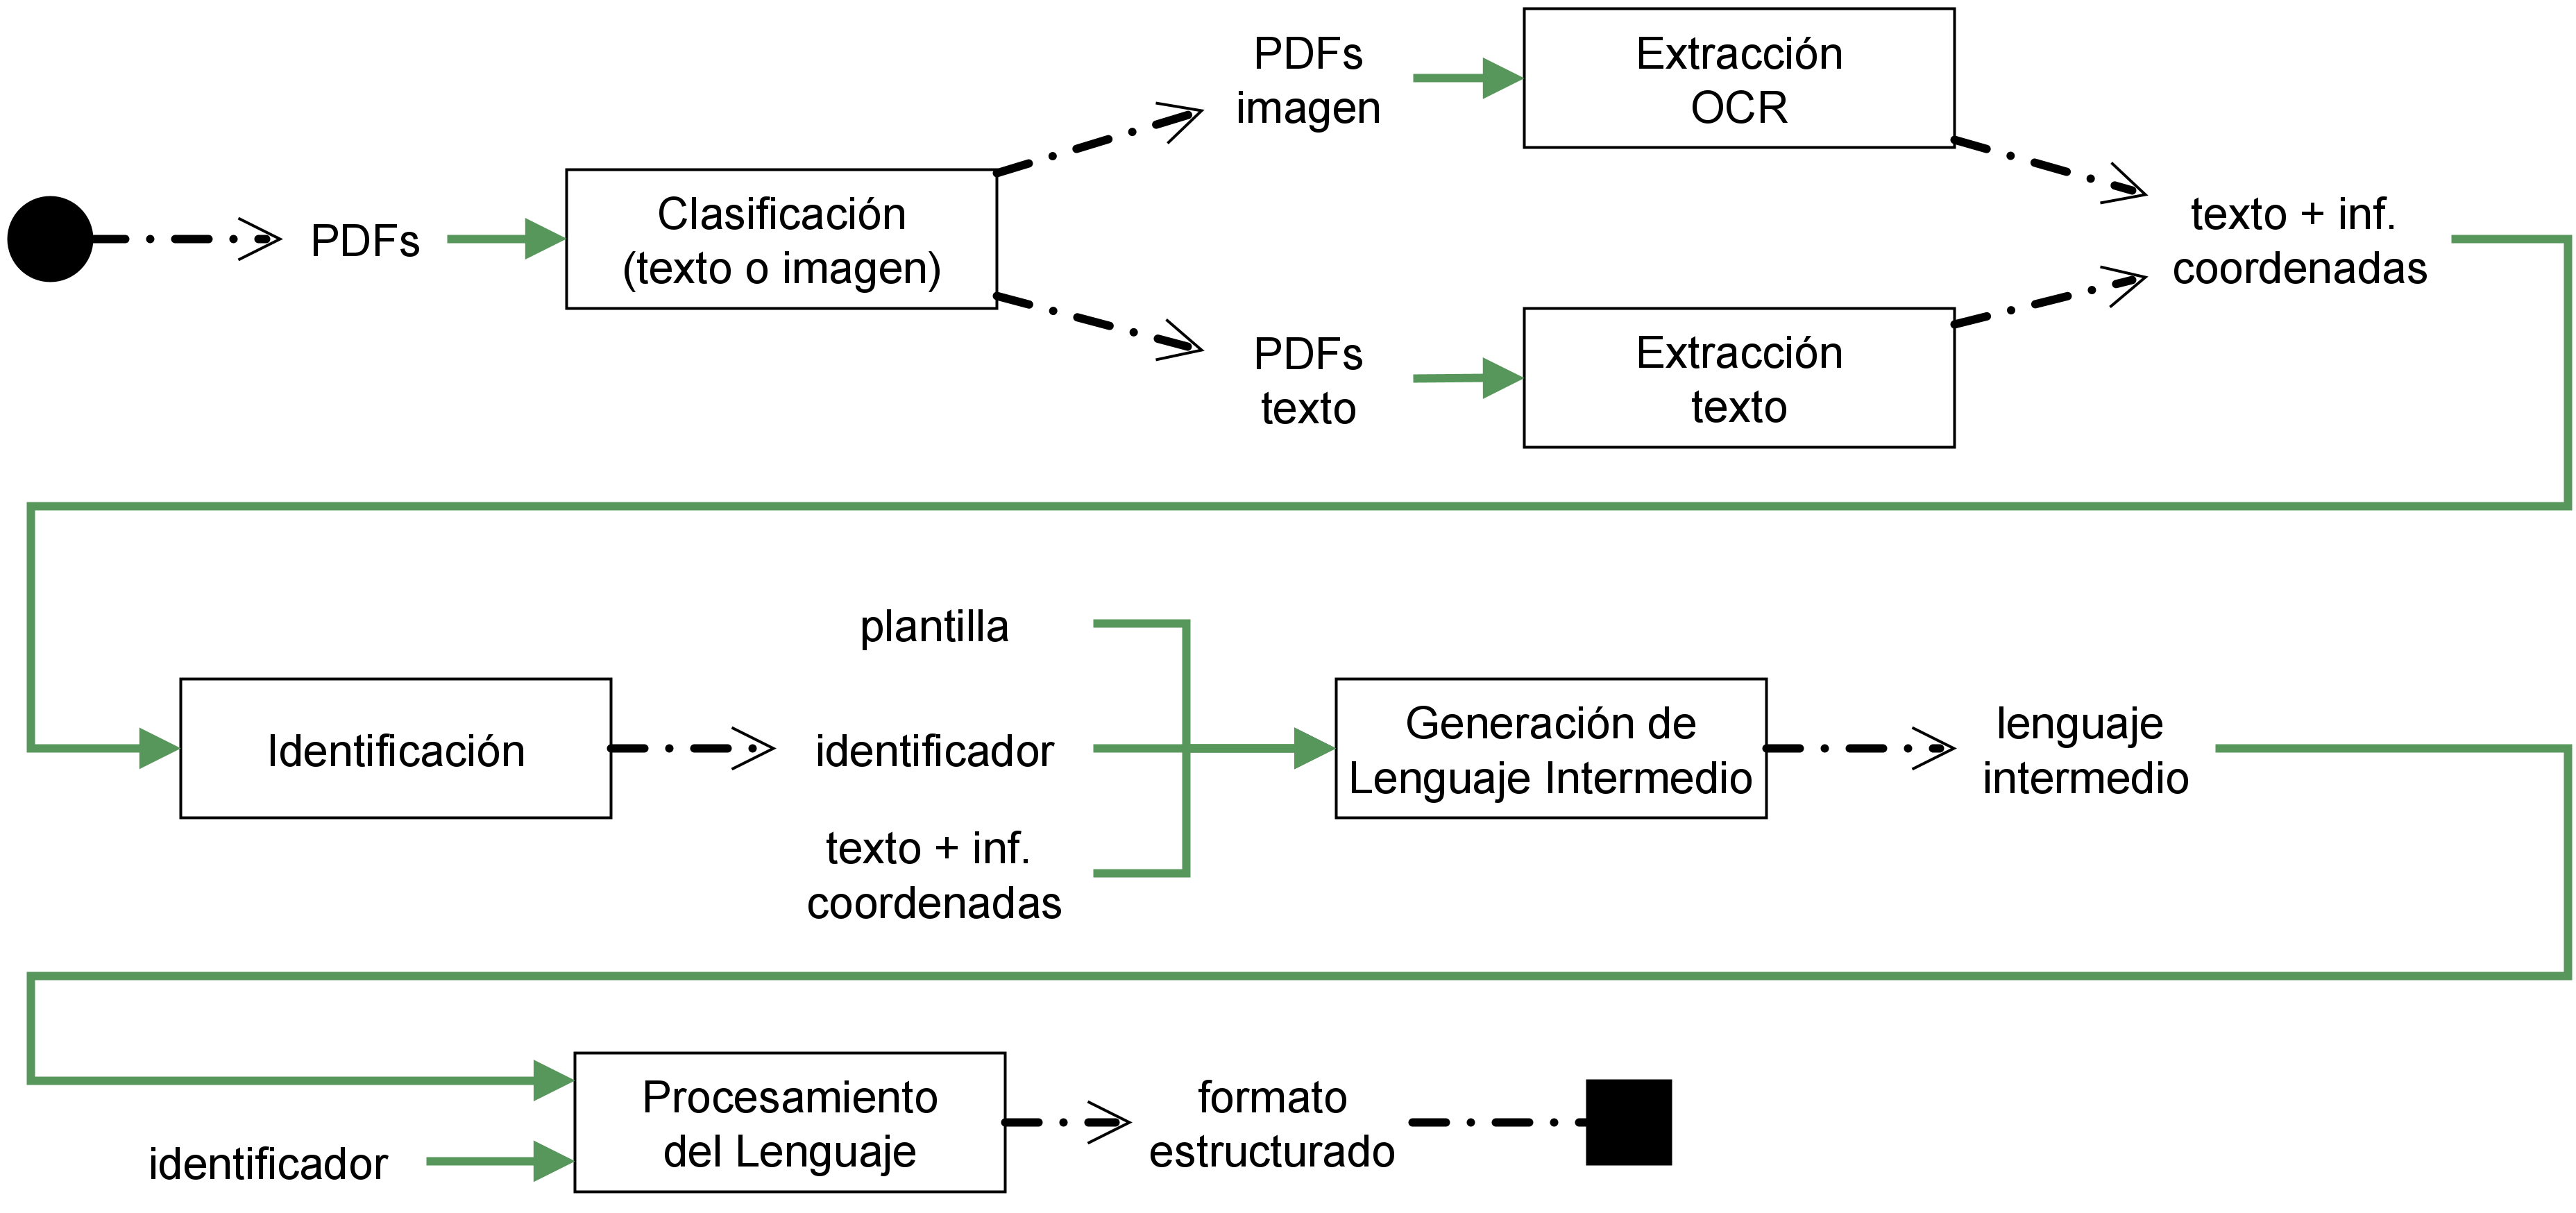
\includegraphics[width=1.0\textwidth]{imaxes/h-implementacion/vision-general-del-sistema-2}
    \caption{Visión general del pipeline del sistema}
    \label{fig:vision-general-del-sistema}
\end{figure}

El proceso comienza cuando se proporcionan al sistema un nuevo conjunto de ficheros PDF. La primera acción realiza la clasificación, según el tipo contenido de los PDF sean páginas con texto o con imágenes. El sistema mantiene el estado interno en base a la creación de los ficheros respetando un esquema de rutas particular.

A continuación se procede a la extracción de la información de los documentos. Además del propio texto, directamente visible, se genera la información de coordenadas que se utilizará para seleccionar los contenidos relevantes.

El proceso sigue con la identificación de los documentos con el objetivo de poder seleccionar la plantilla correcta, si está dada de alta en el sistema. 

Con toda la información obtenida se puede comenzar la generación del lenguaje intermedio de cada página. Para ello, la información de entrada está formada por la plantilla, el código del identificador encontrado y el texto con las coordenadas de la etapa de extracción.

Por último se transforma el lenguaje intermedio y se genera toda la información de salida del sistema. El identificador es utilizado en la  selección del parser necesario para transformar el documento. Cuando los procesos de análisis sintáctico han finalizado para los documentos, todos los datos de salida son movidos a un directorio de resultados y se genera la marca de finalización del tratamiento.

El componente referido como engine o motor se ocupa de conducir todas estas actividades, invocando uno a uno los scripts correspondientes a cada tarea y haciendo evolucionar el trabajo.

\subsection{Creación de un nuevo trabajo}

Si bien la imagen \ref{fig:vision-general-del-sistema} representa el flujo de datos a nivel general, para comenzar el tratamiento se sigue un proceso formalizado en tres pasos. 

Primero el Sistema Externo solicita un identificador para el nuevo job. En ese momento el motor genera el código y lo utiliza para crear las rutas de directorios necesarias para ubicar los resultados de cada etapa. El identificador se obtiene de la fecha UTC actual concatenando segundos y nanosegundos. Se recurre al comando \verb|date| para ello, como se muestra en \ref{lst:creacion-job-id}).

\begin{lstlisting}[language=bash,caption={Obtención del identificador de un trabajo},label=lst:creacion-job-id]
job_id=$(date -u +%s%6N)
\end{lstlisting}

Utilizando el identificador, el Sistema Externo forma el path donde deberá depositar el fichero comprimido. Tras realizar la copia, se le debe indicar al motor que comience el procesamiento del trabajo para el id deseado.

\subsection{Clasificación de los ficheros}

Como primera acción para tratar correctamente los fichero se realiza un saneamiento de los nombres. Aplicar un nombrado homogéneo evita problemas en la construcción de las rutas en el sistema de ficheros. También se descartan los directorios que el fichero comprimido facilitado pudiera contener. El esquema de nombrado para los ficheros utiliza los números naturales desde el 1 y de forma creciente.

Los PDF recibidos deben ser clasificados dependiendo de su contenido. En unos casos es posible utilizar directamente el texto del documento. Para los restantes se procederá a utilizar el procedimiento OCR, como se ha explicado anteriormente. La clasificación se realiza por medio de un test de extracción de texto y se busca una respuesta positiva en la salida.

En \verb|extract-text.sh| se trata cada fichero PDF de tal manera que por cada uno se obtiene su número de páginas. La extracción de texto se realiza página a página, generando como salida un fichero individual para cada una. Desde este punto y para todos los demás procesos los documentos se tratan también página por página hasta llegar al procesamiento del lenguaje intermedio que recibe un único fichero para todas las páginas del documento. En \ref{lst:extraccion-text-inicial} se puede ver el cálculo del número de páginas y la instrucción de extracción.

\begin{lstlisting}[language=bash,caption={Extracción tentativa del texto},label=lst:extraccion-text-inicial]
last_page="$(pdfinfo $line | grep 'Pages:' | cut -c 7- | sed 's_ *__')"
for ((page=1; page<=$last_page; page++))
do
    pdftotext -f $page -l $page -layout "$line" "$n-$page_number.txt"
done
\end{lstlisting}

Cuando un documento no contiene texto, el fichero de la información extraída únicamente almacena caracteres de salto de página, \verb|0x0C|, que son introducidos por el propio \verb|pdftotext|. Estos casos pueden ser localizados mediante un editor hexadecimal, como se muestra en \ref{lst:deteccion-salto-pagina}. En el fragmento, tanto si se ejecuta el cuerpo del \verb|if| como del \verb|elif|, la página se trata de un caso de imagen y el fichero es movido al directorio para los casos de imagen.

\begin{lstlisting}[language=bash,caption={Detección del salto de página},label=lst:deteccion-salto-pagina]
if [ "$(hexdump -e '1/1 "%02X\n"' $i | tr '\n' ' ')" = '0C ' ]
then
    mv $i $base_image_dir
elif [ "$(hexdump -e '1/1 "%02X\n"' $i | tr '\n' ' ')" = '0C * ' ]
then
    mv $i $base_image_dir
fi
\end{lstlisting}

\subsection{Extracción de datos}

Previamente al proceso OCR, el script \verb|extract-images.sh| se encarga de extraer las imágenes contenidas en los ficheros seleccionados en el paso anterior. En este proceso se recupera la información original contenida en el PDF, no se trata simplemente de una \emph{foto} de la página, sino que se utiliza la herramienta \verb|pdfimages| con el flag \verb|-j|. Si las imágenes presentes en el PDF fueron almacenadas en formato JPEG, con este flag se conseguirá recuperar la información sin realizar transformaciones, ya que el formato PDF soporta la codificación JPEG de forma nativa por medio de los filtros DCTDecode y JPXDecode \cite[23]{adobe_book_iso32000-1}. Además, al no requerir transformación la extracción es muy rápida. La situación descrita es la más habitual cuando un escáner profesional digitaliza un número de páginas y crea un PDF final.

El siguiente paso obtiene la información de coordenadas de los casos de texto, nuevamente con \verb|pdftotext|. Se generan los ficheros XHTML cuando se invoca la herramienta con el flag \verb|-bbox-layout|. En \ref{lst:extraccion-text-coord} se muestra un extracto del contenido típico que luego será procesado por el generador de código intermedio. Como se puede apreciar, se identifican la palabras individuales y la línea a la cual pertenecen.

\begin{lstlisting}[language=XML,caption={Extracción de texto con información de coordenadas},label=lst:extraccion-text-coord]
<flow>
    <block xMin="1594.583333" yMin="461.616667" 
            xMax="2148.275000" yMax="496.304167">
    <line xMin="1594.583333" yMin="461.616667" 
            xMax="2148.275000" yMax="496.304167">
        <word xMin="1594.583333" yMin="464.608333" xMax="1690.916667" 
                yMax="495.441667">Fecha</word>
        <word xMin="1700.183333" yMin="464.608333" xMax="1739.083333"   
                yMax="495.441667">de</word>
        <word xMin="1748.350000" yMin="464.608333" xMax="1939.116667" 
                yMax="495.441667">facturación:</word>
    </line>
</block>
\end{lstlisting}

Completada la extracción de texto se da paso al proceso de OCR. El script \verb|image-apply-ocr.sh| recorre el directorio donde están almacenadas las imágenes recuperadas y se invoca a Tesseract con la instrucción que se puede ver en el código \ref{lst:invocacion-de-tesseract}.  Se indican varios parámetros importantes. Debe utilizar utilizar los conjuntos de entrenamiento para contenido en castellano (\verb|-l spa|), ya que los documentos están en este idioma. El número de \acrlong{ppp} se fija a 300 (\verb|--dpi 300|) ya que es un tamaño recomendado que las imágenes deben tener para que el proceso OCR tenga calidad suficiente. Tesseract dispone de varios algoritmos para interpretar el layout de documento. En este caso, al trabajar directamente con las coordenadas, no es necesario tener en cuenta el layout y se le indica que capture la máxima información posible independientemente del orden (\verb|--psm 11|). Por otra parte existe un fichero de configuración, apuntado por la variable \verb|$tessconfig_file| que contiene la directiva para activar la salida en formato hOCR, \verb|tessedit_create_hocr 1|.

\begin{lstlisting}[language=XML,caption={Extracción de texto con información de coordenadas},label=lst:invocacion-de-tesseract]
tesseract $file_path "$outputbase" \
    -l spa \
    --dpi 300 \
    --psm 11 \
    -c page_separator='' \
    --tessdata-dir "$tessdata_dir" \
    $tessconfig_file
\end{lstlisting}

Se puede ver una muestra del formato hOCR en el fragmento \ref{lst:salida-hocr-tesseract}. En el atributo \verb|title| de las palabras se puede ver que aparecen las coordenadas en píxeles respecto al tamaño de la imagen. También hay un indicador de confianza, \verb|x_wconf| que indica la certeza que asigna Tesseract a la identificación de la palabra en particular.

\begin{lstlisting}[language=XML,caption={Fragmento de la salida hOCR de Tesseract},label=lst:salida-hocr-tesseract]
<div class='ocr_page' id='page_1' 
    title='image "input/1627762529247627/based-image/1/1-000.jpg"; 
    bbox 0 0 2480 3509; ppageno 0'>
  <div class='ocr_carea' id='block_1_1' title="bbox 83 141 810 200">
    <p class='ocr_par' id='par_1_1' lang='spa' 
        title="bbox 83 141 810 200">
      <span class='ocr_line' id='line_1_1' title="bbox 83 141 810 200; 
          baseline 0.001 -16; x_size 59; 
          x_descenders 15; x_ascenders 15">
        <span class='ocrx_word' id='word_1_1' title='bbox 83 144 370 185; 
            x_wconf 96'>SALGADO</span>
        <span class='ocrx_word' id='word_1_2' title='bbox 390 141 701 200; 
            x_wconf 93'>Congelados,</span>
      </span>
\end{lstlisting}

\subsection{Identificación}

% TODO si se cambia implementación a SQLite, cambiar explicación.

Los documentos se identifican para poder asociales una plantilla. El mecanismo utilizado consiste en buscar en la información extraída un dato que se considere único para la familia de documentos. Para las facturas tratadas un dato único es el NIF o CIF del emisor, pero podría seleccionarse cualquier dato dependiendo del dominio. Los identificadores están almacenados en los ficheros \verb|id-nif-iva.txt| y \verb|id-cif.txt| en formato \acrshort{csv} en el directorio de datos del sistema.

El script \verb|identify-grep.sh| se encarga de realizar todo el proceso. Primero se leen todos los identificadores por medio de la función \verb|read_identifiers()|, tal como se puede ver en \ref{lst:lectura-de-identificadores}. Los datos leidos son incorporados a un array.

\begin{lstlisting}[language=bash,caption={Lectura de identificadores},label=lst:lectura-de-identificadores]
read_identifiers() {
    while IFS= read -r line; do
        # Add id if line has contents
        [ ! -z $line ] && ids_+=("$(echo -n $line | sed 's_._.*&_g' | cut -c 3-)")
    done < $1
}
\end{lstlisting}

A continuación se obtiene la lista de ficheros para los cuales se ha extraído información y se iteran buscando ocurrencias de los identificadores conocidos, En \ref{lst:identifica-documentos} se le indica a \verb|grep| que tenga en cuenta solo los casos en los que el patron abarque una palabra completa (\verb|-w|), y que cambie la salida habitual por otra con el recuento de ocurrencias (\verb|-c|).

\begin{lstlisting}[language=bash,caption={Identificación de los documentos},label=lst:identifica-documentos]
for file in $files; do
  for id_ in "${ids_[@]}"; do
    if [ "$(grep -w -c "$id_" $file)" -ge 1 ]; then
      #echo 'Found id: "'$id_'" in file: "'$file'"'
      echo $id_ | sed -E 's_\*|\.__g' > $dir_name/$number.id
      break
    fi
  done
done
\end{lstlisting}

Cuando se encuentra un identificador válido, se registra el el directorio del documento con un fichero que tiene por nombre el número del documento y la extensión \verb|id|. Por último se finaliza el bucle y se continua con el siguiente documento.

\subsection{Plantillas y regiones}

% TODO completar significado de los campos que no son de coordenadas
% TODO is_global
% TODO page
% TODO doc_pages

Las plantillas contienen la información de coordenadas de las regiones de interés seleccionadas para el modelo de documento. En el ejemplo de código \ref{ejemplo-plantilla} se ver que para almacenar esta información se utiliza el formato JSON. Además de las coordenadas en si mismas, se utilizan otras claves para dar más flexibilidad a la información y poder tratar casos como los documentos de OVH. La clave \verb|id| que aparece al comienzo se utiliza para asociar con los identificadores de los documentos. Luego el array \verb|regions| contiene la colección de regiones existentes en el modelo. Se utiliza \verb|type| para identificar el tipo de región, \verb|yMin| y \verb|yMax| para las coordenadas horizontales. Los límites verticales se almanenan en el array de columnas \verb|cols|. En el caso de regiones con una única columna se utiliza igualmente el array pero con un único elemento.

\noindent\begin{minipage}{.45\textwidth}
\begin{lstlisting}[language=Java,caption=Comienzo de la plantilla,frame=tlrb]{Name}
{
  "id": "A48941488",
  "is_global": false,
  "regions": [
    {
      "page": "0",
      "type": "R2",
      "doc_pages": "all",
      "yMin": 1112,
      "yMax": 1278,
      "cols": [
        {
          "xMin": 144,
          "xMax": 429
        },
        ...
\end{lstlisting}
\end{minipage}\hfill
\begin{minipage}{.45\textwidth}
\begin{lstlisting}[language=Java,caption=Región T1,frame=tlrb]{Name}
    {
      "page": "0",
      "type": "T1",
      "doc_pages": "all",
      "yMin": 1281,
      "yMax": 2524,
      "cols": [
        {
          "xMin": 76,
          "xMax": 546
        },
        {
          "xMin": 860,
          "xMax": 1906
        }
        ...
    \end{lstlisting}
\end{minipage}

Es un formato homogéneo que para representar todas las regiones. Las primeras plantillas fueron creadas a mano durante el desarrollo utilizando el programa de edición de imágenes GIMP \footnote{\url{http://www.gimp.org.es/}}.

\subsection{Generación del lenguaje intermedio}
% TODO describir la implementación en etapas, como el diagrama general
    % TODO Concepto de línea de identificación
    % TODO Asignación de palabras a regiones
    % TODO información de bounding box
% TODO mostrar el código intermedio
% TODO introducir el problema de indentificar las líneas
% TODO explicar se utiliza el algoritmo de Hough en los ejemplos donde es efectivo
% TODO explicar mejora en el algoritmo para asignación de palabras a regiones para cumplir con el requisito no funcionar de mantener los tiempos contenidos

\subsection{Procesamiento del lenguaje intermedio}
% TODO explicar como es la estructura general de Flex / Bison
% TODO mostrar las modificaciones introducidas
% TODO explicar la carga dinámica de librerías
% TODO Mencionar que el modelo de plugins permite entregar al cliente solo los modelos comprados
% TODO mostrar como es el formato de un fichero Flex y también Bison
% TODO Mostrar como se utiliza la librería para generación de ficheros JSON
% TODO Mencionar el pretty printing con jq
% TODO explicar como es el flujo de información y por qué los terminales y no terminales llevan un tipo de dato en Bison

\subsection{Un engine modular}
% TODO Detalle de la estructura de directorios considerada
% TODO Se imita un modelo de procesamiento en batch
% TODO Se generan códigos de identificación de los jobs recibidos. También marca final.

El motor del sistema es el componente implementado en Bash. Esta decisión se tomó para facilitar el manejo de los ficheros dentro de la estructura de directorios. Además se utilizan herramientas en la consola, que sería más engorroso utilizar desde otros lenguajes de programación.

\section{Compilación y despliegue}

\subsection{Makefile}
% TODO mostrar el Makefile

\subsection{Ansible}
% TODO mostrar script Ansible

\subsection{Docker}
% TODO Mostrar fichero de configuración Docker y su uso

% TODO valorar si incluir capítulo o sección de pruebas. O, al menos, de pruebas realizadas.

\section{Editor de coordenadas}

